\section{Methods}\label{sec:method} % 4 pages

We start with a brief description of our AMG framework. 
Algebraic multigrid (AMG) has been a popular method for solving linear systems
of elliptic partial differential equations, especially for large sparse systems.
The linear system can be written as
\begin{equation}
 Ax = b
\end{equation}
in which, $A \in R^{n \times n}$, $x$ and $b \in R^{n}$.

AMG consists of a setup and a solve phase. During the setup phase, \textit{aggregation} is applied to the equivalent 
graph $G$ of the matrix $A$. Every row of the matrix $A$ is considered as a node in the Graph $G$ and there is an edge between 
nodes $i$ and $j$ if entry $(i,j)$ is nonzero in $A$. Let's say there are $n$ nodes in the graph $G$.
By doing the aggregation on them, $m$ nodes will be chosen as \textit{roots} such that $m < n$ and the rest of the nodes of 
the graph will be assigned to them.
%\textit{2-distance maximal independent set} is used as the aggregation method from \cite{bell2012exposing} by some modifications.
For our implementation we have used \textit{maximal independent set} as the aggregation method.

The prolongation matrix $P \in R^{n \times m}$ will then be defined based on this aggregation. If node $i$ is assigned to root 
$j$, then $P(i,j) = 1$, otherwise it is $0$. The restriction operator $R \in R^{m \times n}$ is then made by transposing $P$.
The prolongation operator has two applications. It can interpolate a vector $v \in R^m$ to $v' \in R^n$, such that $m < n$.
The restriction operator does the reverse task; takes $w \in R^n$ to $R^m$.
The other purpose of $P$ and $R$ is creating a smaller version of the left-hand side matrix $A$, which is called \textit{coarsening}:

\begin{equation}
 A_c = R * A * P
\end{equation}
such that $A_c \in R^{m \times m}$.

Progressively coarser versions of the matrix are created during the setup phase.
An AMG hierarchy of $L+1$ levels consists of three categories of operators:
\begin{enumerate}
 \item Coarse Matrices ($As$)
 \item Prolongation Matrices ($Ps$)
 \item Restriction Matrices ($Rs$)
\end{enumerate}
The coarse matrices are created similar to $A_c$ for each level:
\begin{equation}
 As[l+1] = Rs[l] * As[l] * Ps[l],\ l = 0, 1, 2, ..., L-1
\end{equation}

For this paper, \textit{smoothed aggregation AMG (SA-AMG)} is used from \cite{treister2015non}, for which the prolongation ($P_t$) and restriction
operators ($R_t$) are smoothed by
\begin{equation}
 P = (I - \omega QA^{F})P_t, \ \ \ R = R_t(I - \omega A^{F}Q)
\end{equation}
where $Q$ is a the inverse of the diagonal of A and $\omega$ is the damped Jacobi parameter and $A^F$ is the filtered matrix of $A$.

The second step of AMG is the solve phase. To solve the linear system $Ax = b$, we start with an initial guess for $x$.
Then, we use two methods to reduce the error:
\begin{enumerate}
 \item Relaxation
 \item Coarse-grid Correction.
\end{enumerate}

%Three iterations of damped Jacobi is being applied on $x$ to reduce the high frequency error. Then, the AMG hierarchy will be used to reduce the low-frequency error
%by the coarse-grid correction. Finally, again 3 iterations of damped Jacobi will be applied to the solution vector $x$.

The setup phase is usually more expensive than the solve phase.
%They can be compared in figure \ref{fig:solvesetup} in section \S\ref{sec:results}.
We want to avoid doing at least some parts of the setup phase whenever it is possible,
at the cost of a low (and in some cases no) increase in the solve time.
This will be our goal in the three strategies that are explained in the next section.

\subsection{AMG as a preconditioner}

While AMG can be used directly as a solver for our target problem, using it as a preconditioner
for Conjugate Gradients makes it far more robust, especially given the complexity of our target
meshes (see Figure\ref{fig:mesh}). The pseudocode for using AMG as a preconditioner with CG is
given in Algorithm~\ref{alg:pcg}.

\begin{algorithm}[ht] 
  % v-cycle 
  \caption{Multigrid-preconditioned CG} \label{alg:pcg} 
  \begin{algorithmic}[1]
    \Require rhs and guess
    \Ensure  solution
    \While {not converged} 
    \State $\bs{h} = A \bs{p}$ 											%\Comment $~~\quad\quad\quad\quad\mathcal{O}(Ng_p)$
    \State $\rho_r = (\rho, \bs{r})$								%\Comment $~~\quad\quad\quad\quad\mathcal{O}(N)~~~$
    \State $\alpha = \rho_r / ( \bs{p}, \bs{h} )$		%\Comment $~~\quad\quad\quad\quad\mathcal{O}(N)~~~$
    \State $\bs{u} = \bs{u} + \alpha\bs{p}$					%\Comment $~~\quad\quad\quad\quad\mathcal{O}(N)~~~$
    \State $\bs{r} = \bs{r} - \alpha\bs{h}$					%\Comment $~~\quad\quad\quad\quad\mathcal{O}(N)~~~$
    \State Convergence Test
    \State $\rho = M\bs{r}$ 												\Comment AMG V-cycle %$\quad\mathcal{O}(Ng_p)$
    \State $\beta = (\rho, \bs{r}) / \rho_r$				%\Comment $~~\quad\quad\quad\quad\mathcal{O}(N)~~~$
    \State $\bs{p} = \rho + \beta\bs{p}$						%\Comment $~~\quad\quad\quad\quad\mathcal{O}(N)~~~$
    \EndWhile
  \end{algorithmic}
\end{algorithm}

As previously mentioned, the main downside of using AMG--with or without PCG--for our target problem is
the variation of the diffusion coefficient. This effectively means that the high cost of the AMG setup
is not offset by a sufficiently high number of corresponding solves. By using AMG as a preconditioner
along with PCG, we can update the preconditioner--the multigrid hierarchy--in a lazy fashion,
effectively lowering the effective cost of AMG setup. Of course using a {\em stale} preconditioner can
be less efficient and can increase the number of iterations needed for convergence. We study this
trade-off and consider three different strategies in order to get the overall best runtime.
Note that the overall runtime will involve both the AMG setup as well as the cost of the PCG solves,
therefore there is an incentive to reduce the number of AMG setups, even if it marginally increases
the number of PCG iterations for convergence. We will now discuss the different strategies for lazy
updates of the AMG hierarchy.

%There are two ways to use AMG to solve a linear system $Ax = b$: AMG as a solver, AMG as a preconditioner. The former is very sensitive
%to the changes to the matrix $A$, but the second one is not and this paper takes advantage of this fact and uses preconditioned
%conjugate gradient (PCG) to solve the system, in which AMG is the preconditioner. 

% Let's say we want to solve some similar linear systems, $Ax = b$, $B_1x = b$, $B_2x = b$, ... and so on, in which $B_1$ is made
% by slightly changing the values of $A$. Also, $B_2$ is similarly created by updating the values of $B_1$ by a small change and
% so on. All of them have the same nonzero structure.
% The setup phase of the AMG can be expensive. In the case of solving similar linear systems, three different strategies are
% examined in this paper to keep the cost of the setup phase lower than a complete new setup, at the cost of longer solve phase,
% but saving some time in overall.
% First strategy is to use the whole AMG hierarchy but only update the fine matrix $As[1]$ by $B_1$.
% The second one is updating all $As$ matrices, but keep $Ps$ and $Rs$ from before.
% Finally, the third experiment is updating $As$ only locally and keeping $Ps$ and $Rs$ unchanged.

\subsubsection{Strategy 1: Reuse the same AMG hierarchy}

The first and simplest strategy is to simply use the same AMG hierarchy and only update the input matrix $As[0]$
with the updated matrix (Figure~\ref{fig:str1and2}, left).
One can see from Algorithm~\ref{alg:pcg} that the multigrid hierararchy ($M$) from the previous matrix can be reused.
In this scenario, PCG will use the updated matrix $A$ and so will the fine-grid of the AMG hierarchy.
But the coarse grid operators along with the restriction and prolongation operators will not be recomputed.
Effectively we will not incur an additional setup cost. We only create the updated matrix.
The number of iterations taken by PCG will be higher,
especially as the diffusion coefficients start to vary significantly from the original operator.
However marginal increase in the number of iterations is still cheaper than the cost associated with the AMG setup,
so this is likely to be faster. For long-running simulations, our heuristic is to update the AMG hierarchy by a fresh
setup when the number of iterations becomes \texttt{2x} the number of iterations taken by the first matrix.
In practice this approach works reasonably well, and the number of solves per setup is increased sufficiently to keep
the overall runtime low.

\begin{figure}[ht]
 \centering
 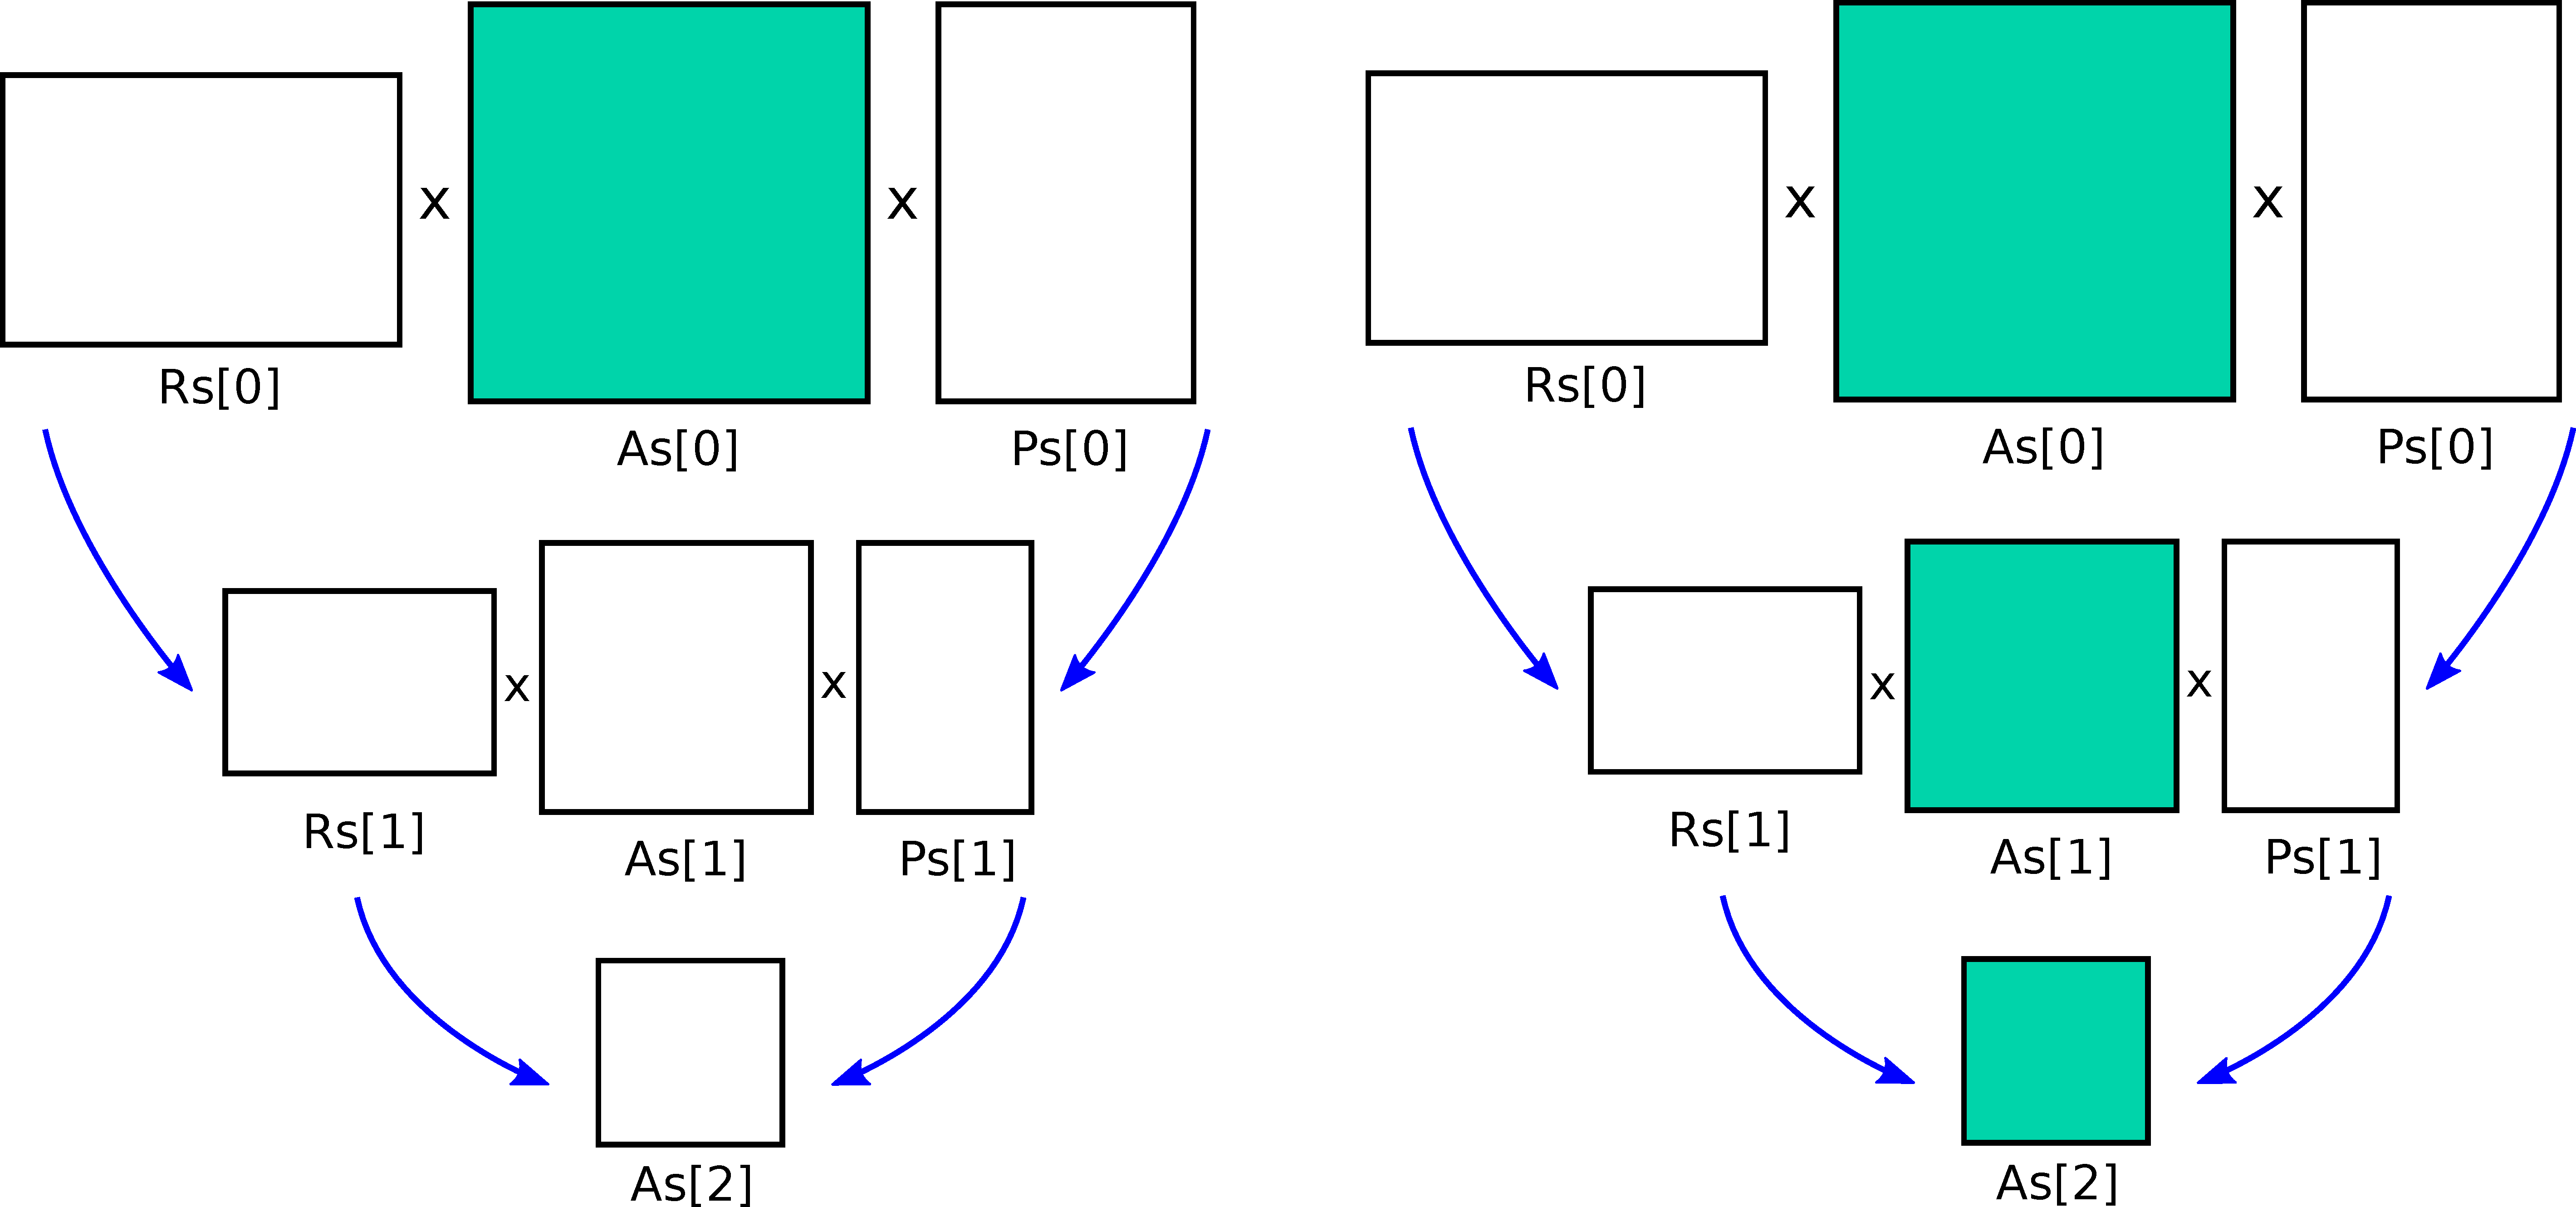
\includegraphics[width=10.5cm,height=5cm]{./figures/strategy1and2.pdf}
 \caption{This figure shows the multigrid hierarchy with 3 levels. Green boxes show which parts should be updated.
          (left) Strategy1: only update As[0].
          (right) Strategy2: update all coarse matrices ($As$).}
 \label{fig:str1and2}
\end{figure}


% As explained before, the AMG hierarchy consists of coarse matrices $As[1]$, $As[2]$, ..., $As[L]$, the prolongation matrices
% $Ps[1]$, $Ps[2]$, ... and $Ps[L-1]$ and the restriction matrices $Rs[1]$, $Rs[2]$, ... and $Rs[L-1]$.
% In our first experiment, we create the AMG hierarchy based on the first left-hand side (LHS) matrix $A$.
% Then, a new left-hand side matrix $B_1$ is created by updating the values of A. The only part of the hierarchy that is being
% updated is $As[1]$, all the rest is unchanged. Then, $B_1x = b$ will be solved and two parameters will be measured: number of vcycle
% iterations in the AMG solve phase and also the time that it takes to update the hierarchy and solve the system. We want the number
% of iterations to increase relatively small, and don't want to spend much time to update the hierarchy. So, a balance between
% these two measurements is expected. The same experiment is being done on $B_2$ which is made by slightly changing the values
% of $B_1$ and so on.

\subsubsection{Strategy 2: Keep the same structure, only update As}

While the previous case works well for many problems, it does not perform very well when there
is large variation in the diffusion coefficients. We observe that variations in the diffusion
coefficients do not affect the overall structure of the matrix.
Therefore, we can use the aggregation from the previous AMG setup and simply update the coarse grid operators.
In other words, we will keep the same aggregations, and therefore the restriction and prolongation operators,
but update the coarse grid operators (Figure~\ref{fig:str1and2}, right). Unlike the previous case, we do have to pay a cost for
re-computing the coarse-grid operators but this is not as expensive as a full AMG setup.
At the same time, the convergence for this approach should be better than Strategy 1,
especially for problems with large variations. 

% In the second experiment, $As[1]$ is replaced by $B_1$. Then, $As[2]$ is changed by $Rs[1] * As[1] * Ps[1]$ and so on.
% This way, all the $As[1]$, $As[2]$, ..., $As[L]$ will be updated.
% This experiment obviously takes more time to update the hierarchy but
% since more parts of the hierarchy is updated based on $B_1$ than the first experiment, so it should take less number
% of iterations in the solve phase.

\subsubsection{Strategy 3: Only update local: No Communication}

% Next experiment is similar to the previous one, but instead of multiplying $Rs[1] * As[1] * Ps[1]$ normally, only local parts of
% $Rs[1]$ and $As[1]$ and $Ps[1]$ will be used to update the diagonal blocks of $As[2]$ from the previous hierarchy and still use
% the non-diagonal blocks of $As[2]$ from before. The result of this experiment stands in the middle of the previous two experiments.

While Strategy 2 works well in the sequential case, it is not the most efficient while computing in parallel.
This is mainly due to the need to perform matrix multiplications in parallel to compute the coarse
grid operator $A_c = RAP$. The communication required can become a bottleneck,
especially as the coarser operators start to get dense. Therefore, as a final approximation,
in the parallel case, we only update the local block of the coarse grid operators and do not incur
any communication costs (Figure~\ref{fig:str3}). The finest level $As$ is updated completely because it is simply replaced by
the updated matrix and does not require any matrix-matrix product. While this can affect convergence slightly, for the most part this simply
behaves like Strategy 2, but is more efficient for large-scale parallel cases.

\begin{figure}[ht]
 \centering
 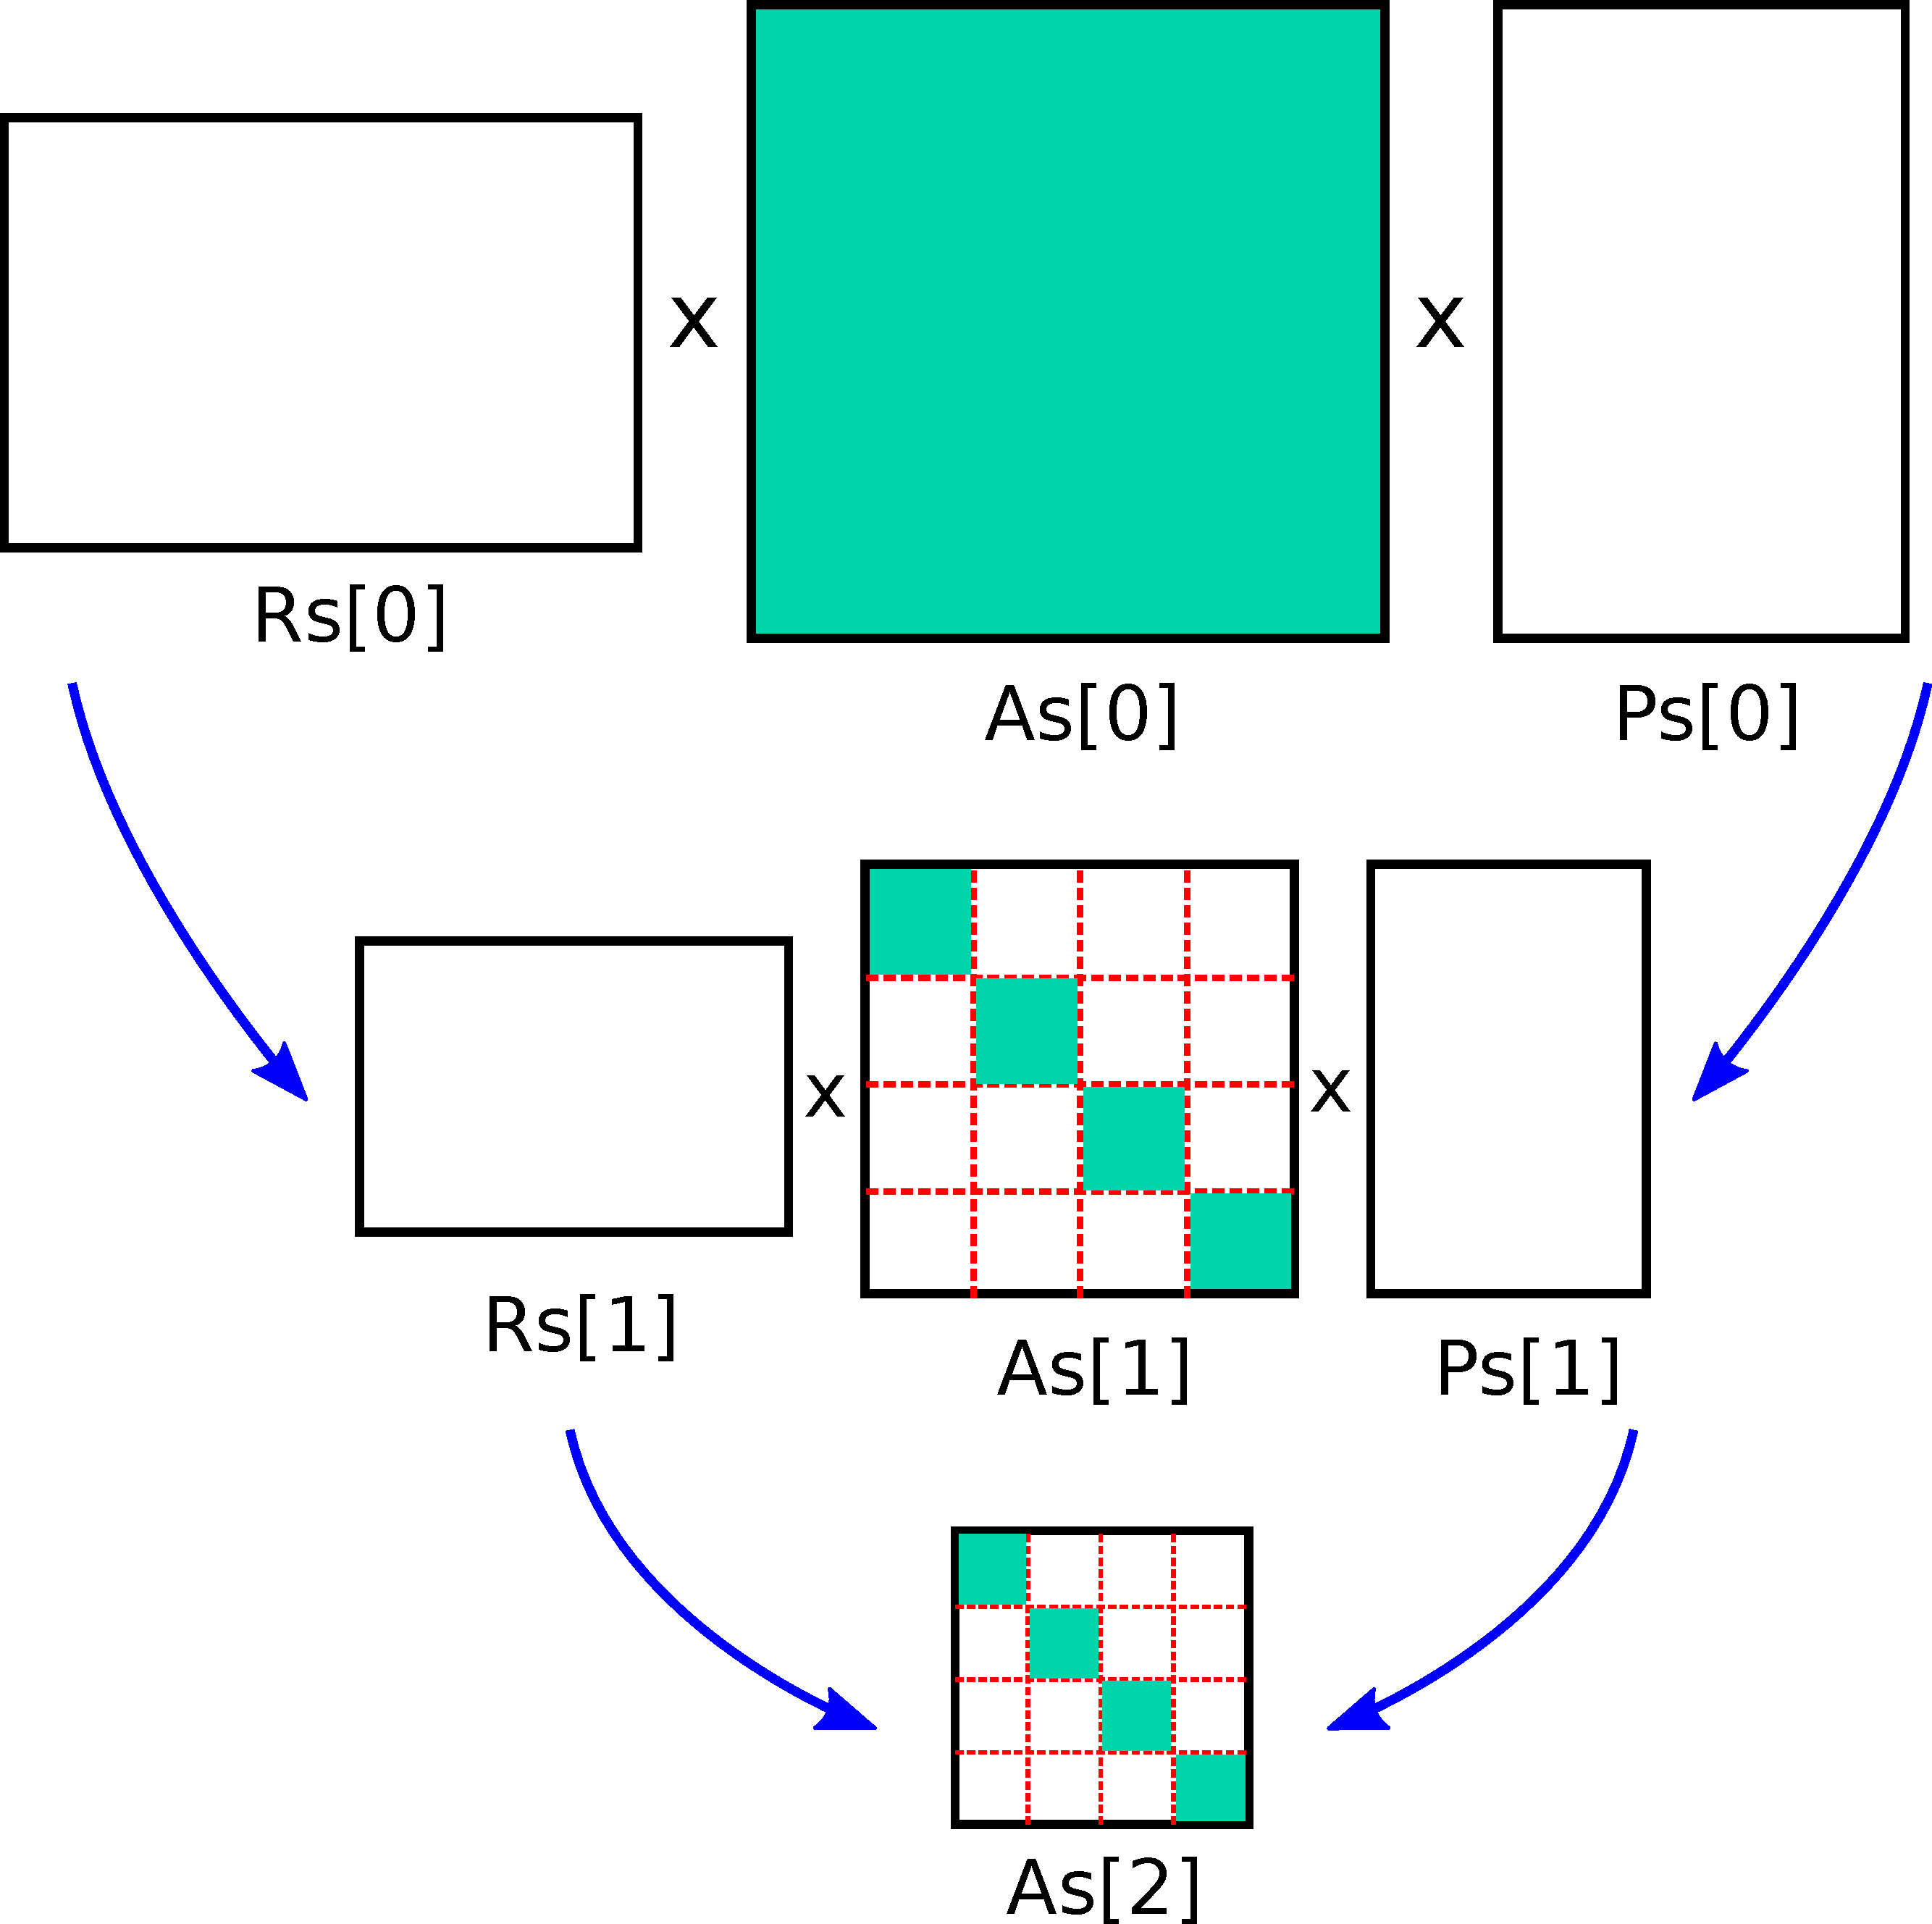
\includegraphics[width=5.2cm,height=5cm]{./figures/strategy3.pdf}
 \caption{Strategy3: Update the diagonal blocks of coarse matrices ($As$) to avoid the communication required
          for matrix-matrix product while performing the coarsening operation ($A_c = RAP$)}
 \label{fig:str3}
\end{figure}
